\documentclass[11pt,a4paper]{article}
\usepackage{acl2015}
\usepackage{times}
\usepackage{url}
\usepackage{latexsym}
\usepackage{graphicx}
\usepackage[none]{hyphenat}
\usepackage[ampersand]{easylist}
\ListProperties(Hide=100, Hang=true, Progressive=3ex, Style*=- , Style2*=$\circ$ )

\title{Text Mining en Social Media\\
M\'aster Big Data Analytics - Curso 2016 / 2017\\
Universitat Polit\`ecnica de Val\`encia\\
\hfill \break
\large Detecci\'on de g\'enero y variedad de idioma en textos extra\'idos de la red social Twitter (datos \textit{PAN-AP'17})
}

\author{Christian Ferrer Fas \\
{\tt chferfa@inf.upv.es} \\}

\date{13/07/2017}

\renewcommand{\thefootnote}{\fnsymbol{footnote}}

\begin{document}
\sloppy
\maketitle

\begin{abstract}

A continuaci\'on, se describe un problema del mundo real consistente en detectar ciertas caracter\'isticas acerca de los autores de textos publicados en redes sociales (concretamente su g\'enero y su variedad de idioma), y se detallan las diferentes acciones que se han llevado a cabo para proporcionar una soluci\'on al mismo.\\
La soluci\'on presentada se basa, grosso modo, en aplicar una serie de t\'ecnicas de \textit{text mining} sobre el \textit{dataset} proporcionado para generar un conjunto de caracter\'isticas que permita, posteriormente, entrenar un modelo de \textit{machine learning} que sea capaz de determinar, ante la llegada de un nuevo texto, ciertas caracter\'isticas sobre el autor del mismo (su g\'enero y su variedad de idioma).\\
A lo largo de la tarea, se pone de relevancia la importancia que tienen ciertas decisiones iniciales sobre el resultado final (entendiendo este como el \textit{accuracy} del modelo entrenado). Las decisiones m\'as importantes se resumen en: aplicar los m\'etodos de preprocesado m\'as adecuados al \textit{dataset} proporcionado, seleccionar el vocabulario m\'as discriminante posible (el uso de pesos \textbf{tf-idf} ha marcado la diferencia en este aspecto) y seleccionar el m\'etodo de \textit{machine learning} m\'as adecuado al tipo de caracter\'isticas a estudiar (los candidatos m\'as adecuados son \textbf{Support Vector Machine} y \textbf{Random Forest}).

\end{abstract}

\section{Introducci\'on}

De forma general, el problema de \textbf{Author Profiling} consiste en detectar ciertas caracter\'isticas del autor de un texto, a partir de caracter\'isticas presentes en el propio texto, tales como el estilo de escritura, expresiones o palabras empleadas, etc.
A continuaci\'on, se presentan dos problemas de \textbf{Author Profiling} a resolver sobre un mismo \textit{dataset}.
El \textit{dataset} est\'a extra\'ido de la red social \textbf{Twitter} y los problemas a resolver consisten en:\\

\begin{easylist}
& Determinar el g\'enero (hombre o mujer) del autor de cada \textit{tweet} a partir del contenido del mismo.
& Determinar la variedad de idioma (argentina, chilena, colombiana, mexicana, peruana, venezolana o espa\~{n}ola) del autor de cada \textit{tweet} a partir del contenido del mismo.
\end{easylist}

\section{Dataset}

El \textit{dataset} proporcionado cuenta con las siguientes caracter\'isticas:\\

\begin{easylist}
& Est\'a separado en dos conjuntos: \textit{training} y \textit{test}.
& Cada muestra, tanto de \textit{training} como de \textit{test}, est\'a constituida dentro de un fichero \textit{XML} que contiene todos los textos de los \textit{tweets} de un mismo autor. El nombre del fichero representa el identificador \'unico de cada autor.
& Las etiquetas de cada muestra, tanto de g\'enero como de variedad, se encuentran en un fichero \'unico y est\'an asociadas a cada una de las muestras por medio del identificador \'unico del autor.\\
\end{easylist}

En cuanto a las dimensiones del \textit{dataset}, tanto en el conjunto de \textit{training} como en el de \textit{test}, cada una de las muestras est\'a compuesta por el texto de 100 \textit{tweets} diferentes de un mismo autor.\\
El conjunto de \textit{training} contiene 2800 muestras, mientras que el conjunto de \textit{test} contiene 1400 muestras (la mitad).\\
Las muestras est\'an distribuidas de forma equitativa entre las dos caracter\'isticas a estudiar: g\'enero y variedad. De este modo, el conjunto de \textit{training} contiene 1400 muestras de cada g\'enero (200 muestras de cada variedad por cada g\'enero) y 400 muestras de cada variedad (200 muestras de cada g\'enero por cada variedad), como se puede observar en la siguiente gr\'afica:

\begin{center}
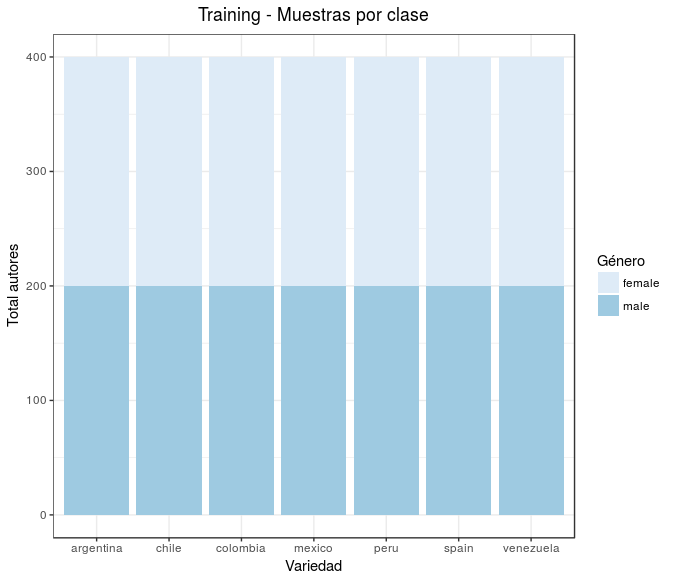
\includegraphics[width=\linewidth]{total_tweets_training.png}
\end{center}

De forma equivalente, el conjunto de \textit{test} contiene 700 muestras de cada g\'enero (100 muestras de cada variedad por cada g\'enero) y 200 muestras de cada variedad (100 muestras de cada g\'enero por cada variedad), como se puede observar en la siguiente gr\'afica:

\begin{center}
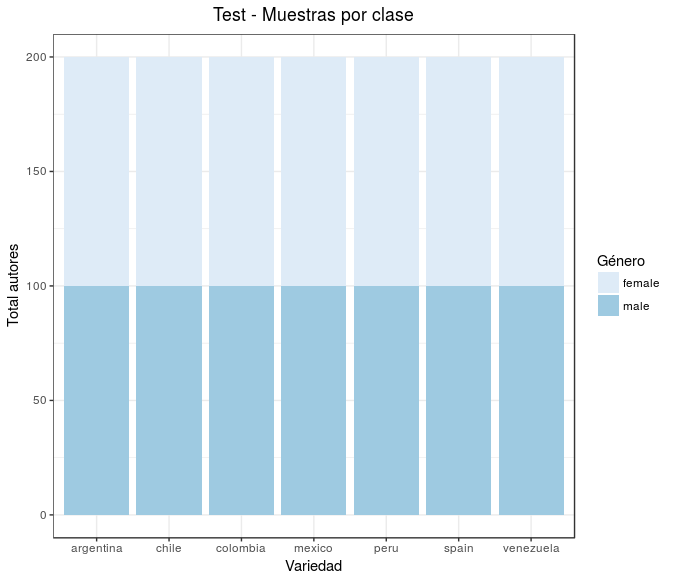
\includegraphics[width=\linewidth]{total_tweets_test.png}
\end{center}

Por tanto, la distribuci\'on de las muestras est\'a perfectamente equilibrada entre las dos caracter\'isticas a estudiar.\\
Adem\'as, las muestras tienen caracter\'isticas similares en cuanto a cantidad de palabras en total y cantidad de palabras por \textit{tweet}. Este aspecto no est\'a distribuido equitativamente de forma perfecta como los anteriores aspectos, pero igualmente est\'a muy bien balanceado, como se puede apreciar en las siguientes gr\'aficas del conjunto de \textit{training}:

\begin{center}
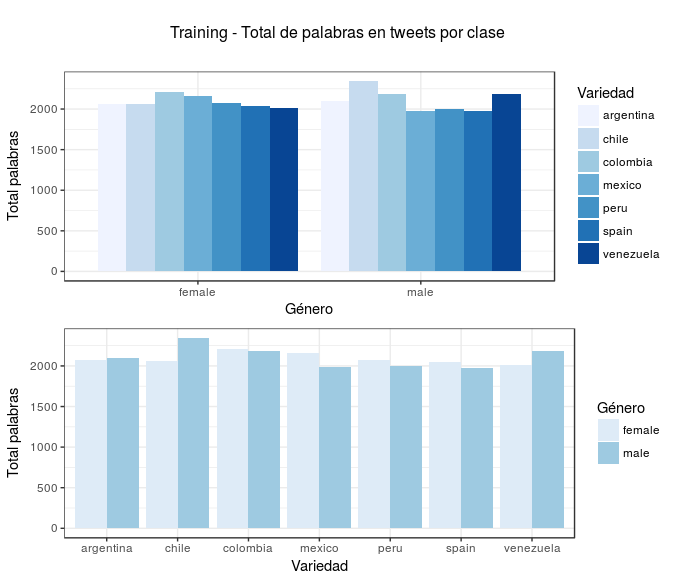
\includegraphics[width=\linewidth]{total_words_training.png}
\end{center}

\begin{center}
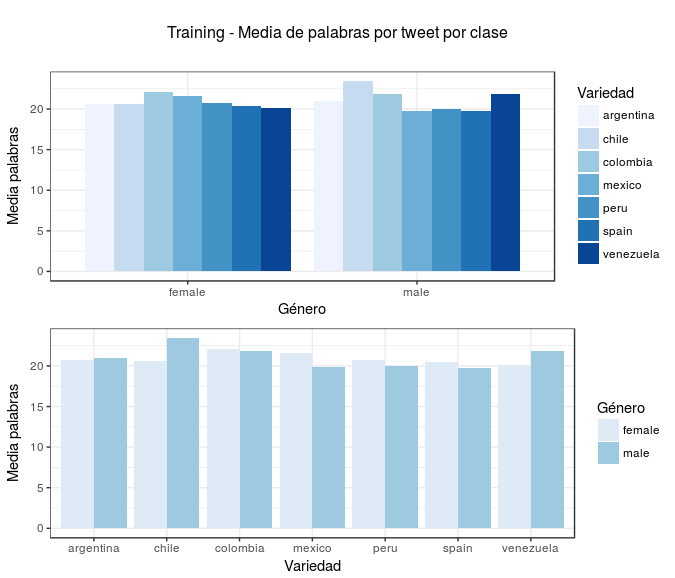
\includegraphics[width=\linewidth]{mean_words_training.png}
\end{center}

La distribuci\'on de palabras en los \textit{tweets} del conjunto de \textit{test} es muy similar, en t\'erminos relativos, a la que se ha mostrado para el conjunto de \textit{training}.\\
El hecho de disponer de un \textit{dataset} tan equilibrado entre las caracter\'isticas a estudiar, reduce dr\'asticamente el problema de desbalanceo que podr\'ia influir negativamente en las t\'ecnicas de \textit{machine learning} a aplicar sobre el mismo.

\section{Propuesta del alumno}

Para resolver ambos problemas (detecci\'on del g\'enero y detecci\'on de la variedad) se ha decidido aplicar el mismo tipo de preprocesado sobre los datos, as\'i como la misma t\'ecnica de \textit{machine learning} para el aprendizaje del modelo, variando algunos aspectos m\'inimos de un problema a otro (el tama\~{n}o del vocabulario). Esta decisi\'on se basa en el tiempo l\'imite disponible para resolver los dos problemas, sin embargo, ser\'ia m\'as id\'oneo realizar un an\'alisis por separado para cada caso, pues cada uno de ellos se podr\'ia abordar mejor aplicando un preprocesado diferente sobre los datos, dada la naturaleza de cada problema.\\
El proceso global consiste en los siguientes 3 pasos generales:\\

\begin{easylist}
& Obtenci\'on del vocabulario a partir de las muestras de \textit{training}:
&& Preprocesado de los textos de los \textit{tweets} y separaci\'on por clases.
&& Obtenci\'on de las palabras m\'as frecuentes para cada clase.
&& Obtenci\'on de los pesos \textbf{tf-idf} para las palabras m\'as frecuentes con respecto a todas las clases.
&& Obtenci\'on las palabras con mayor peso \textbf{tf-idf}: este conjunto de palabras, de tama\~{n}o configurable, constituye el vocabulario.
& Obtenci\'on de las bolsas de palabras para los conjuntos de \textit{training} y de \textit{test}, mediante el vocabulario generado.
& Obtenci\'on del modelo de \textit{machine learning} mediante \textbf{Random Forest}:
&& Preparaci\'on de los datos de las bolsas de palabras para el entrenamiento y el test del modelo.
&& Entrenamiento del modelo.
&& Test del modelo.
&& Evaluaci\'on del modelo.\\
\end{easylist}

El preprocesado de los datos incluye opciones para convertir todas las palabras a min\'usculas, eliminar signos de puntuaci\'on, eliminar n\'umeros, eliminar acentos, eliminar \textit{stop words} (tanto obtenidas con la librer\'ia \textbf{tm} para idioma \textit{es}, como proporcionadas adicionalmente) y normalizar espacios en blanco. Los resultados obtenidos son extraordinariamente variables en funci\'on del preprocesado que se aplique sobre los datos, por lo que estas opciones de preprocesado son altamente configurables para facilitar las sucesivas pruebas.\\
Se han evaluado dos m\'etodos para seleccionar las palabras a incluir en el vocabulario: obtenci\'on de palabras m\'as frecuentes (por medio de la funci\'on proporcionada \textbf{GenerateVocabulary}) y obtenci\'on de palabras con mayor peso \textbf{tf-idf}. El m\'etodo finalmente empleado en la soluci\'on es, en realidad, una combinaci\'on de ambos m\'etodos consistente en: obtener las \textit{n} palabras m\'as frecuentes de cada clase (conjunto de $n \cdot nclases$ palabras), calcular los pesos \textbf{tf-idf} del conjunto anterior y seleccionar las \textit{m} palabras con mayor peso \textbf{tf-idf}.\\
El empleo del c\'alculo de pesos \textbf{tf-idf} (proporcionado por la librer\'ia \textbf{TidyText}) se basa en otorgar un valor mayor a una palabra cuanto m\'as discriminante es (es decir, el valor ser\'a mayor cu\'anto m\'as frecuente sea en su clase y menos en el resto de clases).\\
Una vez se dispone del vocabulario, se generan las bolsas de palabras para los conjuntos de \textit{training} y de \textit{test}. Este proceso consiste en medir las frecuencias de aparici\'on en cada conjunto de las palabras incluidas en el vocabulario y seleccionar aquellas m\'as frecuentes (junto a su frecuencia).\\
Los datos de las bolsas de palabras se adec\'uan para poder emplearlos en el aprendizaje del modelo de \textit{machine learning} mediante \textbf{Random Forest} (proporcionado por la librer\'ia \textbf{caret}). El modelo entrenado es testeado con los datos de la bolsa de palabras de \textit{test} y evaluado mediante una matriz de confusi\'on, que proporciona el dato del \textit{accuracy}.\\
Para llegar a este proceso, se han ido probando diferentes t\'ecnicas, siendo estas las que mejor resultado han ofrecido. Entre las t\'ecnicas descartadas, se encuentran principalmente las siguientes:\\

\begin{easylist}
& Obtenci\'on de vocabulario basado en \textit{n-gramas}, en lugar de palabras.
& Modelo de \textit{machine learning} mediante \textbf{Support Vector Machine}. Aunque en la literatura se aconseja como el m\'etodo m\'as efectivo para este tipo de problemas, los resultados de las diferentes pruebas han resultado ser mejores en cuanto a \textit{accuracy} empleando \textbf{Random Forest}.
\end{easylist}

\section{Resultados experimentales}

El \textit{baseline} proporcinado es el siguiente, para la medida de \textit{accuracy}:

\begin{center}
\begin{tabular}{|l|l|}
\hline
\multicolumn{1}{|c|}{\textbf{Clase}} & \multicolumn{1}{|c|}{\textbf{\textit{Accuracy}}} \\
\hline \hline
G\'enero & \multicolumn{1}{|r|}{0.6643} \\ \hline
Variedad & \multicolumn{1}{|r|}{0.7721} \\ \hline
\end{tabular}
\end{center}

Se han aplicado las siguientes configuraciones de preprocesado y vocabulario:

\begin{center}
\begin{tabular}{|l|l|l|}
\hline
\multicolumn{1}{|c|}{\textbf{Preprocesado}} & \multicolumn{1}{|c|}{\textbf{G\'enero}} & \multicolumn{1}{|c|}{\textbf{Variedad}} \\
\hline \hline
Min\'usculas & \multicolumn{1}{|c|}{SI} & \multicolumn{1}{|c|}{SI} \\ \hline
Puntuaci\'on & \multicolumn{1}{|c|}{SI} & \multicolumn{1}{|c|}{SI} \\ \hline
N\'umeros & \multicolumn{1}{|c|}{SI} & \multicolumn{1}{|c|}{SI} \\ \hline
Acentos & \multicolumn{1}{|c|}{SI} & \multicolumn{1}{|c|}{SI} \\ \hline
\textit{Stop words} \textbf{tm} & \multicolumn{1}{|c|}{SI} & \multicolumn{1}{|c|}{SI} \\ \hline
\textit{Stop words} adicionales & \multicolumn{1}{|c|}{SI} & \multicolumn{1}{|c|}{SI} \\ \hline
Espacios en blanco & \multicolumn{1}{|c|}{SI} & \multicolumn{1}{|c|}{SI} \\ \hline
\end{tabular}
\end{center}

\begin{center}
\begin{tabular}{|l|l|l|}
\hline
\multicolumn{1}{|c|}{\textbf{Vocabulario}} & \multicolumn{1}{|c|}{\textbf{G\'enero}} & \multicolumn{1}{|c|}{\textbf{Variedad}} \\
\hline \hline
\textbf{n} (frecuencia) & \multicolumn{1}{|r|}{1000} & \multicolumn{1}{|r|}{1000} \\ \hline
\textbf{m} (tama\~{n}o vocabulario) & \multicolumn{1}{|r|}{700} & \multicolumn{1}{|r|}{500} \\ \hline
\end{tabular}
\end{center}

Con el proceso y la configuraci\'on descritos, se han obtenido los siguientes valores de accuracy:

\begin{center}
\begin{tabular}{|l|l|}
\hline
\multicolumn{1}{|c|}{\textbf{Clase}} & \multicolumn{1}{|c|}{\textbf{\textit{Accuracy}}} \\
\hline \hline
G\'enero & \multicolumn{1}{|r|}{0.7343} \\ \hline
Variedad & \multicolumn{1}{|r|}{0.9157} \\ \hline
\end{tabular}
\end{center}

A lo largo de todo el proceso, se han incluido mediciones de los tiempos para cada uno de los pasos computacionalmente m\'as comlejos. A continuaci\'on, de indican estos tiempos (expresados en segundos):

\begin{center}
\begin{tabular}{|l|l|l|}
\hline
\multicolumn{1}{|c|}{\textbf{Acci\'on}} & \multicolumn{1}{|c|}{\textbf{G\'enero}} & \multicolumn{1}{|c|}{\textbf{Variedad}} \\
\hline \hline
Preprocesar y separar & \multicolumn{1}{|r|}{12.5750} & \multicolumn{1}{|r|}{3.5552} \\ \hline
Palabras frecuentes & \multicolumn{1}{|r|}{12.3195} & \multicolumn{1}{|r|}{3.3954} \\ \hline
Pesos \textbf{tf-idf} & \multicolumn{1}{|r|}{0.0030} & \multicolumn{1}{|r|}{0.0050} \\ \hline
Bolsa palabras \textit{training} & \multicolumn{1}{|r|}{169.8910} & \multicolumn{1}{|r|}{132.9490} \\ \hline
Bolsa palabras \textit{test} & \multicolumn{1}{|r|}{88.8420} & \multicolumn{1}{|r|}{65.7310} \\ \hline
Entrenar modelo & \multicolumn{1}{|r|}{76.1590} & \multicolumn{1}{|r|}{62.2180} \\ \hline
Testear modelo & \multicolumn{1}{|r|}{0.2160} & \multicolumn{1}{|r|}{0.1840} \\ \hline
Evaluar modelo & \multicolumn{1}{|r|}{0.0030} & \multicolumn{1}{|r|}{0.0150} \\ \hline
\end{tabular}
\end{center}

\section{Conclusiones y trabajo futuro}

Tras el trabajo realizado se puede observar que la detecci\'on de la variedad es un problema relativamente m\'as sencillo de solucionar que la detecci\'on del g\'enero, a partir de textos publicados en  \textbf{Twitter}. Uno de los posibles motivos puede ser que, debido a que existen palabras aut\'octonas o exclusivas en cada pa\'is (que se emplean en dicho pa\'is y no en el resto), la discriminaci\'on de la variedad usando como caracter\'isticas el empleo de estas palabras ofrece poca probabilidad al error. Sin embargo, no parece existir una caracter\'istica discriminante tan profunda entre las palabras que emplean hombres y mujeres (quiz\'as el problema hubiera sido m\'as sencillo si se tratara de detectar rangos de edad).\\
Ante la dificultad aparente de encontrar palabras que discriminen los g\'eneros, parece razonable pensar que el uso de un vocabulario basado en \textit{n-gramas} podr\'ia ofrecer nuevas posibilidades, ya que permitir\'ia enfocar el aprendizaje del modelo a expresiones propias de cada género.\\
Otro aspecto que se ha podido observar de forma muy notable es la importancia que existe en el preprocesado de los datos, habi\'endose mejorado considerablemente el \textit{accuracy} en la detecci\'on de la variedad al quitar acentos en las palabras. Sin embargo, esto es otro ejemplo donde es posible que un preprocesado m\'as concreto sobre los signos de puntuaci\'on, acentos, etc., podr\'ia permitir al modelo aprender caracter\'isticas m\'as discriminantes para la detecci\'on de la varidad, aprendiendo los estilos de escritura predominantes en cada pa\'is.\\
En cuanto a trabajo futuro, se consideran las siguientes posibilidades:\\
\begin{easylist}
& Preprocesado de emoticonos, principalmente para la detecci\'on del g\'enero.
& Ampliar conjunto de \textit{stop words} adicionales.
& A\~{n}adir informaci\'on externa al vocabulario.
& Expansi\'on de \textit{URL}s, principalmente para la detecci\'on de la variedad \footnote{Esta funcionalidad ya se ha implementado en la soluci\'on, pero no se ha empleado puesto que, al tratarse de una ejecuci\'on secuencial, el tiempo necesario para su ejecuci\'on es muy elevado; por tanto, el trabajo futuro consistir\'ia en realizar una implementaci\'on multihilo, o bien ejecutarlo de forma externa e incorporar los resultados como un \textit{dataset} auxiliar.}.
& \textit{Tunning} de par\'ametros del proceso, desde las opciones de preprocesado hasta los tama\~{n}os del vocabulario.
& M\'etodos de \textit{machine learning} alternativos (profundizar en la parametrizaci\'on de \textbf{Support Vector Machine} y emplear otros m\'etodos, como \textbf{Redes Neuronales Artificiales}).
\end{easylist}

\begin{thebibliography}{}

\bibitem[\protect\citename{Dr. Francisco Manuel Rangel Pardo y Dr. Paolo Rosso}2017]{}
Dr. Francisco Manuel Rangel Pardo y Dr. Paolo Rosso
\newblock 2017
\newblock {\em Material asignatura Text Mining en Social Media}, M\'aster Big Data Analytics, curso 2016/2017
\newblock Universitat Polit\`ecnica de Val\`encia

\bibitem[\protect\citename{The Comprehensive R Archive Network}]{}
{\em The Comprehensive R Archive Network}
\newblock https://cran.r-project.org

\bibitem[\protect\citename{Machine Learning in Python}]{}
{\em scikit-learn}
\newblock {\em Machine Learning in Python}
\newblock http://scikit-learn.org

\bibitem[\protect\citename{Wikipedia }]{}
{\em Wikipedia }
\newblock https://es.wikipedia.org/wiki/Tf-idf

\end{thebibliography}

\end{document}
